% \section{Problem Statement}
\section{Research Scope}
\label{sec:scope}

\jh{To formulate the research scope, we carry out a systematic literature review (SLR) aimed at identifying leading techniques in Android malware detection.
Our literature search encompass major digital libraries, such as the ACM Digital Library and IEEE Xplore.
The search strategy primarily involve using specific keywords such as \textit{android malware detection, android analysis, android malware}, and \textit{malware analysis} to pinpoint pertinent studies.
Additionally, it is supplemented by a manual review of titles and abstracts to exclude papers not specifically focused on Android malware detection.
Ultimately, the comprehensive process yields 258 relevant papers.
}

\begin{figure}[t]
    \centering
    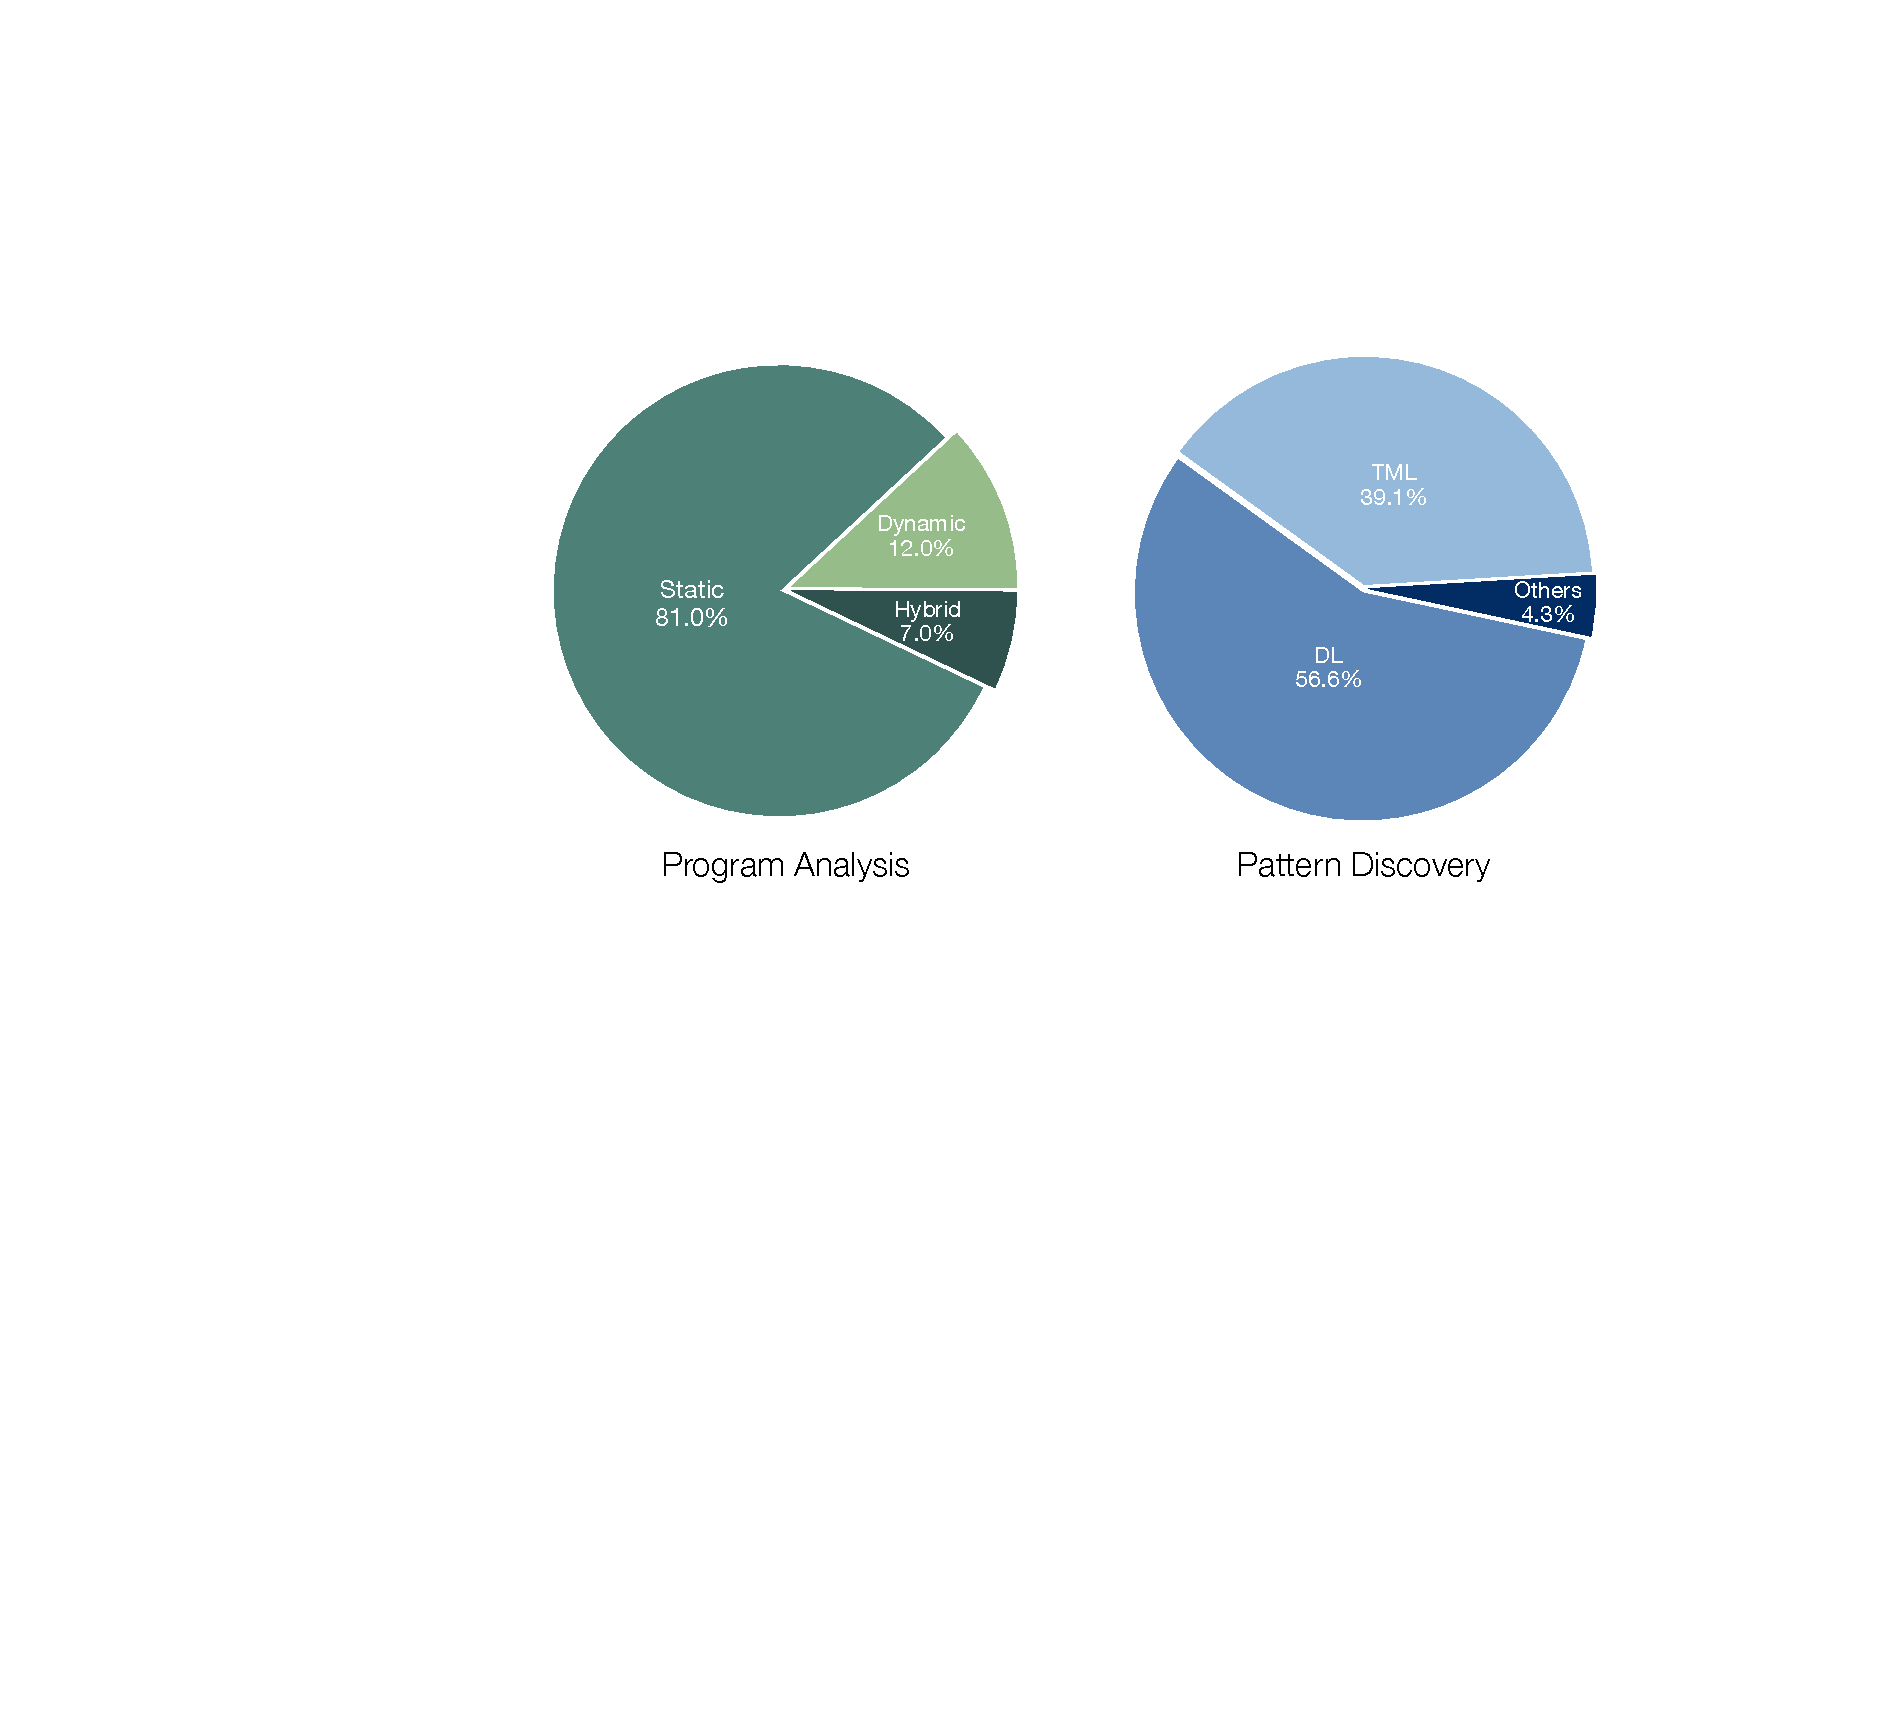
\includegraphics[width=0.6\linewidth]{fig/paper_distribution.pdf}
    \caption{Distribution of investigated approaches since 2011.}
    \label{fig:paper_distribution}
    \vspace{-0.3cm}
\end{figure}
% \jh{This study focuses on \textit{machine learning-based Android malware detection that favors static analysis for feature extraction.}
% To determine the research scope, we conduct a systematic literature review (SLR) to identify the predominant techniques in the field.
% Specifically, program analysis refers to the methods used to extract APK features, while pattern discovery involves the strategies employed to discern malicious patterns.}
\jh{
Figure~\ref{fig:paper_distribution} presents the distribution of predominant techniques, specifically program analysis and pattern discovery, in Android malware detection since 2011.
Program analysis refers to the methods for extracting APK features, while pattern discovery involves the strategies employed to discern malicious patterns.
Notably, static analysis, accounting for 81.0\% of the literature, plays a more significant role than dynamic analysis in APK characterization.
Additionally, machine learning models, including both traditional and deep learning approaches, have gained substantial attention to uncover malicious patterns, being employed in 95.7\% of the studies.

This observation motivates our study towards a focus on \textit{machine learning-based Android malware detection that favors static analysis for feature extraction.}
More specifically, our study is guided by two pivotal questions: \textbf{how can ML models be employed to detect Android malware with static features effectively?} and \textbf{how do existing techniques perform in ML-based Android malware detection?}
}

To address these questions, \jh{we begin with an empirical analysis, concentrating on scrutinizing the detection process used in existing methodologies.}
Next, an in-depth quantitative analysis is conducted on a bunch of representative works to reveal the performance and challenges of current techniques.
Drawing from our investigations, we consolidate our insights and put forth recommendations to facilitate future research.

% \fabio{This reads more like background than research scope.}
% When presented with an Android Package Kit (APK), the objective of Android malware detection is to distinguish malicious apps from benign ones.
% At its core, the malware detection system revolves at least two fundamental steps: extraction of features from the APK and decide whether there are malicious behaviors based on the features. 
%subsequent pattern recognition within its characterization.
%-------------------------------------------------------------------------
% The Android malware detection system involves two fundamental steps: characterizing APKs and recognizing malicious patterns from their characterization.
% In the process of APK characterization, either static or dynamic analysis methods are used to extract features.
% The static analysis employs reverse engineering tools, \textit{e.g.}, Androguard~\cite{androguard}, to disassemble and extract APK features.
% Contrastingly, dynamic analysis characterizes APKs via simulating their execution.
% While this method stands out for revealing accurate behavioral patterns, it is frequently noted for its high resource consumption and extensive time requirements.
%-------------------------------------------------------------------------
% Due to these practical considerations, static analysis has solidified its position as the primary method to characterize APKs.
%-------------------------------------------------------------------------
% To uncover patterns within APK characterization, researchers have historically either formulated detection rules manually~\cite{enck2009lightweight,felt2011android} or turned to machine learning models~\cite{arp2014drebin,wu2019malscan,li2021robust,mclaughlin2017deep,he2022msdroid,wu2021homdroid,xu2020sdac,aafer2013droidapiminer,xu2018deeprefiner} to automatically learn patterns from the features.
% Given the intricate complexities within Android apps, crafting detection rules by hand has become an infeasible task.
%-------------------------------------------------------------------------


%-------------------------------------------------------------------------
% As a result, static analysis and machine learning have emerged as preferred techniques for APK characterization and pattern recognition, respectively.
%-------------------------------------------------------------------------
% \jiahao{detailed search strategy is described in the supplementary material}
%-------------------------------------------------------------------------
% Figure~\ref{fig:paper_distribution} showcases the distribution of predominant techniques in Android malware detection since 2011.
% Evidently, static analysis contributes to 81.0\% of the literature, playing a crucial role in APK characterization. 
% Concurrently, machine learning models have garnered significant attention for pattern recognition, being employed in 95.7\% of the studies.
%-------------------------------------------------------------------------
% \fabio{I somehow feel this statement should arrive earlier and could be integrated in a separate section} \zhenkai{we can mention it earlier, and formally define the research problem here} \jiahao{I understand it, but I want to use the previous paragraph to motive our study. do you have any suggestion how to modify the flow.}
%-------------------------------------------------------------------------
% This study focuses on machine learning-based Android malware detection that favors static analysis for feature extraction.
% More specifically, our study is guided by two pivotal questions: \textbf{how can machine learning models be employed to detect Android malware effectively?} and \textbf{how do existing techniques perform in ML-based Android malware detection?}
%-------------------------------------------------------------------------
% \zhenkai{need deeper research questions}